\section{Graph Skeletal Structure}

The Graph Skeletal Structure is obtained considering the \textit{reduced marker set}, obtained after the reduction from the \textit{full marker set} which has been discussed previously. \\
We model the human skeleton as an undirected graph, where the vertices are the joints and the edges represent connections between consecutive physical body joints.\\
Each edge is associated with a specific weight, the value of which depend on a feature extracted from motion capture data. \\
From this \textit{graph skeletal structure}, we define a mathematical game in which the vertices are the players and the edges model the communication channels (through which movement can propagate) between these players. \\
In figure we can see the \textit{graph skeletal structure} without \textit{non-physical links} and a table with the joints' labels.
For simplicity, the links are without weights.

\begin{figure}[H]
    \centering
    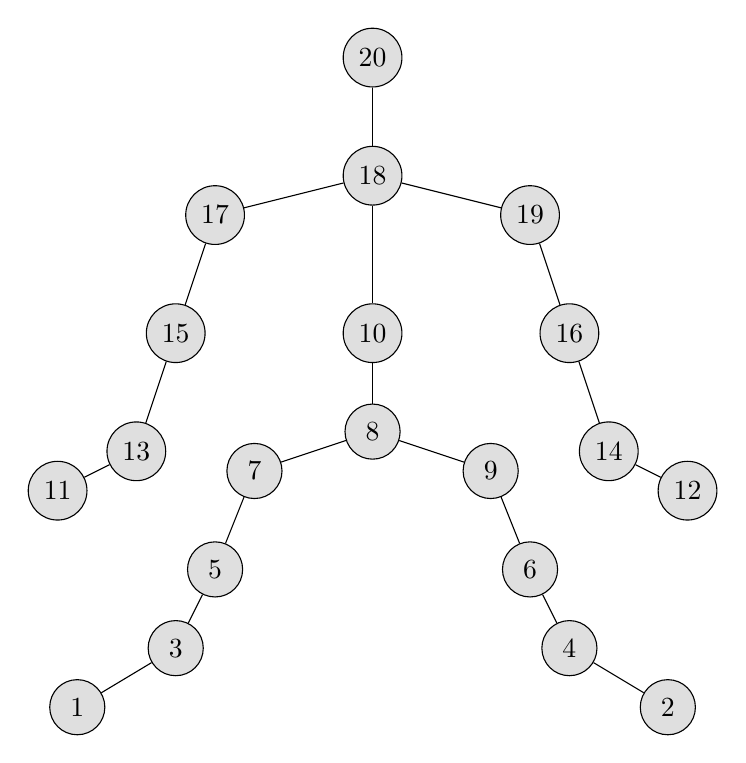
\begin{tikzpicture}
      \node[circle, draw, minimum size=0.7cm] (1) at (1.25,-4.75) [fill=gray!25] {1};
      \node[circle, draw, minimum size=0.7cm] (2) at (8.75, -4.75) [fill=gray!25] {2};
      \node[circle, draw, minimum size=0.7cm] (3) at (2.5,-4) [fill=gray!25] {3};
      \node[circle, draw, minimum size=0.7cm] (4) at (7.5, -4) [fill=gray!25] {4};
      \node[circle, draw, minimum size=0.7cm] (5) at (3,-3) [fill=gray!25] {5};
      \node[circle, draw, minimum size=0.7cm] (6) at (7,-3) [fill=gray!25] {6};
      \node[circle, draw, minimum size=0.7cm] (7) at (3.5,-1.75) [fill=gray!25] {7};
      \node[circle, draw, minimum size=0.7cm] (8) at (5, -1.25) [fill=gray!25] {8};
      \node[circle, draw, minimum size=0.7cm] (9) at (6.5,-1.75) [fill=gray!25] {9};
      \node[circle, draw, minimum size=0.7cm] (10) at (5,0) [fill=gray!25] {10};
      \node[circle, draw, minimum size=0.7cm] (11) at (1,-2) [fill=gray!25] {11};
      \node[circle, draw, minimum size=0.7cm] (12) at (9,-2) [fill=gray!25] {12};
      \node[circle, draw, minimum size=0.7cm] (13) at (2, -1.5) [fill=gray!25] {13};
      \node[circle, draw, minimum size=0.7cm] (14) at (8, -1.5) [fill=gray!25] {14};
      \node[circle, draw, minimum size=0.7cm] (15) at (2.5,0) [fill=gray!25] {15};
      \node[circle, draw, minimum size=0.7cm] (16) at (7.5,0) [fill=gray!25] {16};
      \node[circle, draw, minimum size=0.7cm] (17) at (3,1.5) [fill=gray!25] {17};
      \node[circle, draw, minimum size=0.7cm] (18) at (5,2) [fill=gray!25] {18};
      \node[circle, draw, minimum size=0.7cm] (19) at (7,1.5) [fill=gray!25] {19};
      \node[circle, draw, minimum size=0.7cm] (20) at (5,3.5) [fill=gray!25] {20};
      
      \foreach \source/\dest/\label/\xshiftval in {20/18//0, 18/17//0, 18/19//0, 17/15//0, 15/13//0, 13/11//0, 19/16//0, 16/14//0, 14/12//0, 18/10//0, 10/8//0, 8/7//0, 7/5//0, 5/3//0, 3/1//0, 8/9//0, 9/6//0, 6/4//0, 4/2//0}
        \path (\source) edge node[xshift=\xshiftval] {\label} (\dest);
    \end{tikzpicture}
    \caption{Graph Skeletal Structure}
    \label{fig:graph_skeletal}
  \end{figure}


\begin{table}[H]
  \centering
  \begin{tabular}{|c|c|}
      \hline
      \textbf{Node} & \textbf{Label} \\
      \hline
      1 & right\_foot \\
      2 & left\_foot \\
      3 & right\_ankle \\
      4 & left\_ankle \\
      5 & right\_knee \\
      6 & left\_knee \\
      7 & right\_hip \\
      8 & hip\_centre \\
      9 & left\_hip \\
      10 & spine \\
      11 & right\_hand \\
      12 & left\_hand \\
      13 & right\_wrist \\
      14 & left\_wrist \\
      15 & right\_elbow \\
      16 & left\_elbow \\
      17 & right\_shoulder \\
      18 & shoulder\_centre \\
      19 & left\_shoulder \\
      20 & head \\
      \hline
  \end{tabular}
  \caption{Label of each joint}
  \label{tab:labels_joints}
\end{table}


\subsection{Movement features extraction}
The low-level features extracted for our purpose are \textit{speed}, \textit{tangential acceleration}, and \textit{angular momentum}. \\
While speed indicates how quickly an object is moving, acceleration indicates how rapidly its velocity is changing.\\
Angular momentum provides information about the rotation of an object around a fixed point.\\
By incorporating all three quantities as features, a more comprehensive and detailed view of the overall motion is obtained.

\subsubsection{Speed}
Speed is calculated by finding the change in positions with respect to time through differentiation and then applying a moving average to obtain a more accurate estimate that is less affected by noise.
We calculate this speed as the norm of the velocity vector. \\
The speed of a moving object is a fundamental information in understanding how it moves and how its trajectory might evolve.

\begin{equation}
  \vec{v}(t) = \frac{d\vec{r}}{dt} = \left(\frac{dx}{dt}, \frac{dy}{dt}, \frac{dz}{dt}\right)
\end{equation}

\subsubsection{Tangential Acceleration}
By calculating the derivative of velocity, we can obtain tangential acceleration.
Tangential acceleration is calculated as the norm of the tangential acceleration vector. \\
Tangential acceleration can be used to express specific emotions, styles, and intentions. \\
For instance, rapid acceleration might be associated with energetic and rhythmic movements, whereas a more gradual acceleration could be linked to fluid and delicate motions.

\begin{equation}
  \vec{a}(t) = \frac{d\vec{v}}{dt} = \left(\frac{d^2x}{dt^2}, \frac{d^2y}{dt^2}, \frac{d^2z}{dt^2}\right)
\end{equation}

\subsubsection{Angular Momentum}
The formula we use to calculate angular momentum is:

\begin{equation}
  \vec{L} = \vec{r} \times \vec{p}
\end{equation}

where:

\begin{itemize}
  \item \(\vec{r}\) is the position vector at time \(t\) minus the centre of mass of the whole body
  \item \(\vec{p} = m \vec{v}\) is linear momentum, where:

\begin{itemize}
  \item \textit{m} is the joint mass
  \item \(\vec{v}\) is the velocity
\end{itemize}

\end{itemize}

Analyzing angular momentum can reveal specific patterns of rotation or changes in orientation. \\
These patterns can be used to identify distinctive gestures or movements in activities such as gymnastics or choreography.

\subsection{Cosine similarity}
To calculate the weights of the edges connecting the different joints, we use the \textit{Cosine similarity}. \\
Cosine similarity is a measure of similarity between two vectors, frequently used to gauge how aligned vectors are in space. \\
It returns a value ranging from -1 to 1.
The concept is that similar vectors will have a small angle between them, resulting in a cosine similarity value close to 1. \\
Conversely, dissimilar vectors will have a wide angle and a cosine similarity close to 0.\\
We iteratively calculate the similarity between all the joints connected by an edge.
By doing this, it is possible to compare the directions of the two considered nodes, and thus evaluate if two nodes are associated with
(nearly) the same direction.
\\

After obtaining the weights for each edge of the graph, we then have, for each instantaneous frame, a graph $G$ := ($V$, $E$, $w$), where 
$V$ is the set of $vertices$, $E$ is the set of $edges$ and $w$ is the set of $edge weights$.